\section{Einleitung}
\label{s:intro}

\section{Vorgestellte Technologien}
\label{s:grundlagen}

Im folgenden Kapitel wird einleitend eine kurze Erläuterung über die drei zentralen Begriffe dieser Arbeit gegeben. Besonderer Schwerpunkt ist dabei die Aufschlüsselung der Begriffe und die Erklärung warum Diese in dieser Arbeit einen derartigen Stellenwert besitzen.\\ 

\subsection{IoT}
\label{ss:grundlagen:beispiele}


\subsection{Industrie 4.0}
\label{ss:grundlagen:hardware}


\subsection{SAP}
\label{ss:grundlagen:frequenz}


\section{Allgemeine Funktionsweise Bluetooth Low Energy}
\label{s:funktionsweise}

\noindent Im nachfolgenden Kapitel wird nun ein kurzer Überblick über die Technologie \ac{ble} gegeben. Dabei wird zum einen die Architektur anhand des Protokollstacks und zum anderen die Funktionsweise erläutert.\\   

\subsection{Protokollstack}
\label{ss:funktionsweise:protokollstack}

\begin{figure}[h]
	\centering
	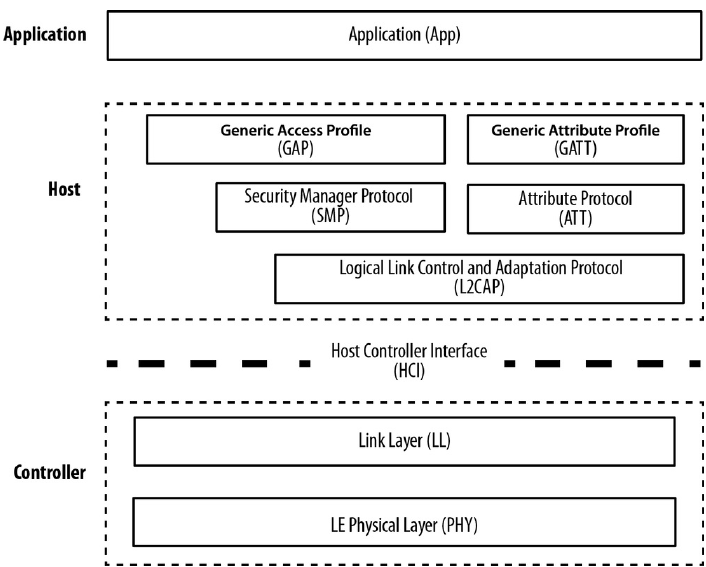
\includegraphics[width=0.9\linewidth]{\figdir/BLE_Protokolstack}
	\caption{\ac{ble} Protokollstack \cite[Seite 16]{Townsend14:GSB}}
	\label{FIG:protokollstack}
\end{figure}

\noindent Die Architektur von \ac{ble} lässt sich anhand des Protokollstacks erkennen. in Abbildung \ref{FIG:protokollstack} ist dieser dargestellt. Besonders auffällig ist, dass er in drei Ebenen unterteilt ist. Der "`Controller"' ist dabei der Bereich, welcher am nächsten an der Hardware sitzt. Hier befinden sich die zwei Lagen "`LE Physical"' und "`Link"'.\\

\noindent Diese beiden Protokolle sind in einer Großzahl von Gerätearchitekturen beheimatet. Das Physical Layer ist dafür vorgesehen, digitale Signale (Bitfolgen) in analoge umzuwandeln. Dieser Schritt wird benötigt, um die \ac{ble} Signale für etwaige Empfänger zugänglich zu machen. Natürlich werden im Physical Layer auch empfangene analoge Signale in digitale umgewandelt. Dieser werden dann im Protokollstack nach oben ins Link Layer weitergereicht. Im Fall von \ac{ble} ist die Schnittstelle für das Senden der analogen Signale die Luft. \ac{ble} sendet daher im Frequenzbereich beginnend bei 2,4GHz bis 2,4835GHz \cite[Seite 7]{RAN:Ble}. Diesen Bereich teilt sich das Protokoll mit anderen wie zum Beispiel Wifi. Um Kollisionen zu vermeiden teilt \ac{ble} den Bereich in 40 Kanäle auf und wechselt während der Verbindung in regelmäßigen Abständen oder bei Übertragungsproblemen den Kanal. Dieser Ansatz nennt sich Frequency Hopping Spread Spectrum \cite[Seite 17]{Townsend14:GSB}.\\      

\noindent Das Link Layer unterscheidet sich in seiner Funktionsweise nicht großartig von dem anderer Kommunikationsprotokolle. Hier werden die Nachrichten die für das  Versenden aus den oberen Schichten ankommen in Pakete gepackt und an das Physical Layer weitergereicht. Dieser Prozess ist für ankommende Pakete natürlich vice versa \cite[Seit 194]{Tanenbaum14:CN}.\\

\noindent Im Link Layer von \ac{ble} wird die Paketgröße festgelegt. Diese lässt seit Version 4.2 eine Payload von 251 Byte pro Paket zu \cite{Gupta:WWW}. Zum Vergleich bei WLAN (IEEE 802.11) kann ein Paket bis zu 2312 Byte groß sein \cite{MTU:WWW}. Daraus lässt sich schließen, dass \ac{ble} einen weitaus geringeren Datendurchsatz als WLAN hat. Allerdings liefert \ac{ble} wiederum andere Vorteile. Auf diese wird in Kapitel \ref{s:vergleich} näher eingegangen.\\

\noindent Das Herzstück des \ac{ble} Protokollstacks bilden die beiden Profile \ac{gap} und \ac{gatt}. Diese befinden sich wie in Abbildung \ref{FIG:protokollstack} zu erkennen im Host Bereich der Architektur. Die beiden Protokolle bilden die Schnittstelle zur tatsächlichen Anwendung mit welcher der Nutzer letzten Endes interagiert.\\

\noindent Das \ac{gap} ist dafür vorgesehen sämtliche Parameter der Verbindung zwischen den Geräten zu verwalten. Vom Verbindungsaufbau bis hin zur Kommunikation werden sämtliche Funktionen von diesem Profil bereitgestellt und abgehandelt.\\

\noindent Im Zuge der jeweiligen Konfiguration kann ein Gerät in \ac{ble} eine der folgenden vier Rollen annehmen:
\begin{itemize}
	\item{Broadcaster (Keine Verbindung)}
	\item{Observer (Keine Verbindung)}
	\item{Central (Verbindung)}
	\item{Peripheral (Verbindung)}
\end{itemize}   

\noindent In \ac{ble} ist es nicht festgeschrieben, dass Geräte ein Verbindung eingehen müssen um Informationen zu erhalten. Die Rollen des Broadcasters und Observers sind sogar ausschließlich ohne feste Verbindung zwischen den Geräten vorgesehen. Diese Funktion wird im allgemeinen gerne von \ac{ble} Beacons verwendet.\\

\noindent Ein Gerät welches als Broadcaster definiert ist sendet dauerhaft einen bestimmten Datensatz. Dabei ist zu keinem Zeitpunkt klar, ob Geräte in Reichweite sind, welche den Datensatz empfangen. Ein Gerät welches diese Daten lesen kann muss als Observer konfiguriert sein. Ein solcher scannt die drei Advertisement Kanäle von \ac{ble} dauerhaft nach Broadcastnachrichten. Falls er eine erhält ließt er diese und verwendet sie. Wichtig ist hierbei, dass der Observer keine Antwort auf eine Nachricht sendet.\\  

\noindent Sollte ein Gerät allerdings eine Verbindung eingehen, dann muss dieses als Central konfiguriert sein. Dies ist die gängigste Form des \ac{ble} Gerätes. So ist beispielsweise jedes Smartphone in der Regel als Central konfiguriert und kann Verbindungen zu Peripherals wie zum Beispiel \ac{ble} Kopfhörern aufnehmen. Dabei ist ein Central in der Regel sogar in der Lage mehrere Verbindungen zu selben Zeit einzugehen.\\

\noindent Ein Peripheral wiederum ist das Gegenstück zum Central, welches seine Verbindungsbereitschaft an sämtliche Geräte in Reichweite signalisiert. Im Fall einer aktiven Verbindung übernimmt das Central die Steuerung des Gerätes unter Berücksichtigung des Funktionsumfangs des Peripherals. \cite[Seite 15]{RAN:Ble}\\

\noindent Das \ac{gap} ermöglicht es einem \ac{ble} Gerät zusätzlich seine Sichtbarkeit und Verbindungsbereitschaft gegenüber anderen Geräten über die Advertisement Kanäle mitzuteilen. Dafür wird auf dem Gerät ein Modus eingestellt welcher anschließend an alle Geräte in Reichweite mitgeteilt wird. Ein Modus ist dabei eng mir der Geräterolle verbunden. Ein Gerät kann folgende Modi annehmen \cite[Seite 16]{RAN:Ble}:
\begin{itemize}
	\item{Broadcast (Rolle: Broadcaster)}
	\item{Nicht zu entdecken (Rolle: Peripheral)}
	\item{Eingeschränkt zu entdecken (Rolle: Peripheral)}
	\item{Normal zu entdecken (Rolle: Peripheral)}
	\item{Nicht verbindbar (Rolle: Alle)}
	\item{Verbindbar (Rolle: Central, Peripheral)}
\end{itemize}   

\subsection{Kommunikation}
\label{ss:funktionsweise:kommunkation}

Todo: Rollen Verbindung und Kommunikation

Nachdem in Kapitel \ref{ss:funktionsweise:protokollstack} der allgemeine Aufbau von \ac{ble} erläutert wurde, wird im nachfolgenden Kapitel auf das Kernelement, die tatsächliche Kommunikation zwischen zwei oder mehreren Geräten von \ac{ble} eingegangen. Dabei werden drei Elemente im besonderen betrachtet: die Bekanntmachung, die Verbindung und der Datenaustausch.\\

\subsubsection{Advertisement}
\label{sss:funktionsweise:advertisement}

Das Advertsement, oder zu deutsch die Bekanntmachung, ist die Funktion, mittels welcher sich Geräte, die bereit sind, sich zu koppeln bei suchenden Geräten bekannt machen. Allerdings kann die Bekanntmachung auch für einen Broadcast von Daten ohne explizites Zielgerät verwendet werden.\\

\noindent Für das Advertisement sind drei der 40 Kanäle, in die der Frequenzbereich auf dem \ac{ism} Band unterteilt ist, reserviert. Ein Gerät kann diese Kanäle nutzen und ein Paket senden, welches verbindungsspezifische Daten bereitstellt. Generell gibt es folgende vier unterschiedliche Pakete, welche somit gesendet werden können:
\begin{itemize}
	\item{ADV\_IND}
	\item{ADV\_DIRECT\_IND}
	\item{ADV\_SCAN\_IND}
	\item{ADV\_NONCONN\_IND}
\end{itemize} 
Das "`ADV\_IND"' Paket sendet eine Bekanntmachung an alle Geräte, die zuhören und gibt bekannt, dass das Gerät bereit ist, sich mit jeglichem Gerät zu verbinden. Im Gegensatz dazu sendet das "`ADV\_DIRECT\_IND"' Paket eine direkte Nachricht an ein bestimmtes Gerät, dass es bereit ist, sich mit genau diesem zu koppeln. Um das zu gewährleisten, enthält die Payload des Paketes die beiden \ac{ble} Adressen der betroffenen Geräte. Diese beiden Pakete lassen auch zu, dass sich die Geräte miteinander verbinden. Die restlichen zwei Pakete lassen dies wiederum nicht zu. So ermöglicht das "`ADV\_SCAN\_IND"' Paket, lediglich einen Broadcast an alle hörenden Geräte zu senden, dass dieses Gerät in Reichweite ist. Es ist also sichtbar für die anderen Geräte. Um jedoch eine Verbindung einzugehen, müssen weitere Schritte unternommen werden. Das letzte Paket teilt allen Geräten in Reichweite mit, dass dieses Gerät nicht für eine Kopplung zu Verfügung steht. Alle Pakete bis auf das "`ADV\_DIRECT\_IND"' Paket können zusätzlich Daten enthalten, die über das Advertisement hinausgehen. Das ermöglicht auch den Einsatz von \ac{ble} Beacons, welche, ohne eine Verbindung einzugehen, Daten an alle Geräte in Reichweite senden können \cite{ADV:WWW}.\\

\subsubsection{Verbindung}
\label{sss:funktionsweise:verbindung}

Nachdem in Kapitel \ref{sss:funktionsweise:linked} erklärt wurde, wie Pakete aufgebaut sind und übertragen werden, gilt es noch zu erläutern, wie eine Verbindung in \ac{ble} abläuft, um diese Pakete tatsächlich transferieren zu können. Nachdem ein Central ein Gerät über das Advertisement gefunden hat, kann es eine Verbindungsanfrage initiieren. In diesem Paket sind drei wichtige Verbindungsparameter angegeben:
\begin{itemize}
	\item{Verbindungsintervall}
	\item{Slave Latenz}
	\item{Überwachungszeitüberschreitung}
\end{itemize}
Das Verbindungsintervall legt die Zeit fest, die zwischen zwei Verbindungsevents verstreicht. Eine Verbindung in \ac{ble} besteht ausschließlich aus derartigen Ereignissen und bleibt solange bestehen, wie diese regelmäßig stattfinden. Bei diesem Intervall gilt es abzuwägen, was wichtiger ist. Je geringer dieses Intervall ist, desto schneller ist die Verbindung. Jedoch verbraucht dieses Verhalten auch mehr Energie. Das Central muss also im Vorhinein festlegen, was für die kommende Verbindung wichtiger ist \cite{CON:WWW}. Die Slave Latenz legt die Nummer der Verbindungsevents an, die der Slave erlaubt ist, zu überspringen, bevor die Verbindung als beendet gilt. Ein weiterer Weg, wie eine Verbindung vorzeitig abgebrochen werden kann, wird durch die Überwachungszeitüberschreitung festgelegt. Bei dieser wird definiert, wie viel Zeit zwischen zwei erfolgreichen Übertragungen verstreichen darf. Sollte es also zu dem Fall kommen, dass über einen längeren Zeitraum erfolglos Pakete versendet werden, wird die Verbindung beendet \cite[Seite 23]{Townsend14:GSB}.\\

\begin{figure}[h]
	\centering
	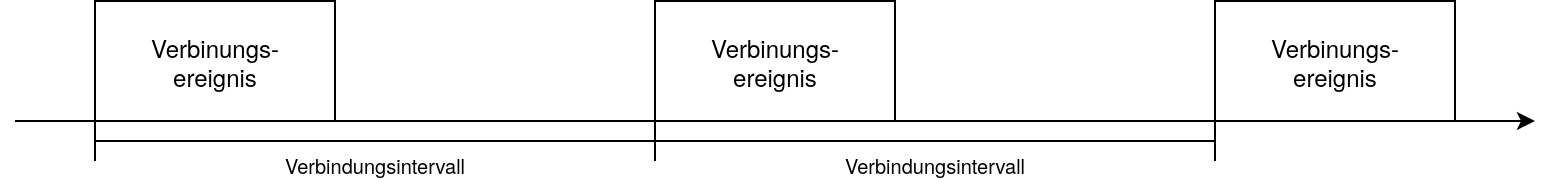
\includegraphics[width=\linewidth]{\figdir/ConEv}
	\caption{Ablauf einer \ac{ble} Verbindung \cite{CON:WWW}}
	\label{FIG:conenv}
\end{figure}

\noindent Wenn das Peripheral die Verbindung annimmt, wird diese, wie in Abbildung \ref{FIG:conenv} dargestellt, aufgenommen. Jedes dieser Ereignisse folgt einem bestimmten Ablauf: zuerst überträgt der Master eine Anfrage an den Slave. Dieser empfängt die Anfrage und verarbeitet diese. Anschließend sendet er eine entsprechende Antwort, die der Master empfängt. Wichtig dabei ist, das der Master nicht nur die Verbindung initiiert, sondern auch sämtliche Anfragen. Nachdem das definierte Verbindungsintervall abgelaufen ist, wird das nächste Verbindungsevent gestartet \cite{CON:WWW}.\\       

\subsection{Anwendungsszenarien}
\label{ss:funktionsweise:anwendungen}

\section{Schnittstellenbeschreibung}
\label{s:interface} 

\subsection{SAP}
\label{ss:interface:sap}

\subsection{BLE}
\label{ss:interface:ble}

\subsection{Anbindungsmöglichkeiten}
\label{ss:interface:connect}

\subsubsection{Bewertung der Möglichkeiten}
\label{sss:interface:connect:eval}

\subsubsection{Administration}
\label{sss:interface:connect:admin}

\section{Vergleich mit anderen gängigen IoT Kommunikationsprotokollen}
\label{s:vergleich} 

\subsection{Vorteile}
\label{ss:vergleich:adv}

\subsection{Nachteile}
\label{ss:vergleich:disadv}

\section{Fazit}
\label{s:fazit}

  
%%% Local Variables: 
%%% mode: latex
%%% TeX-master: "thesis.tex"
%%% End: 
